\section*{Log ud}
Log ud inddeles i en boundary og en dertilhørende controller, som det fremgår af \autoref{fig:MVCLogUd}. 

\begin{figure} [H]
\centering
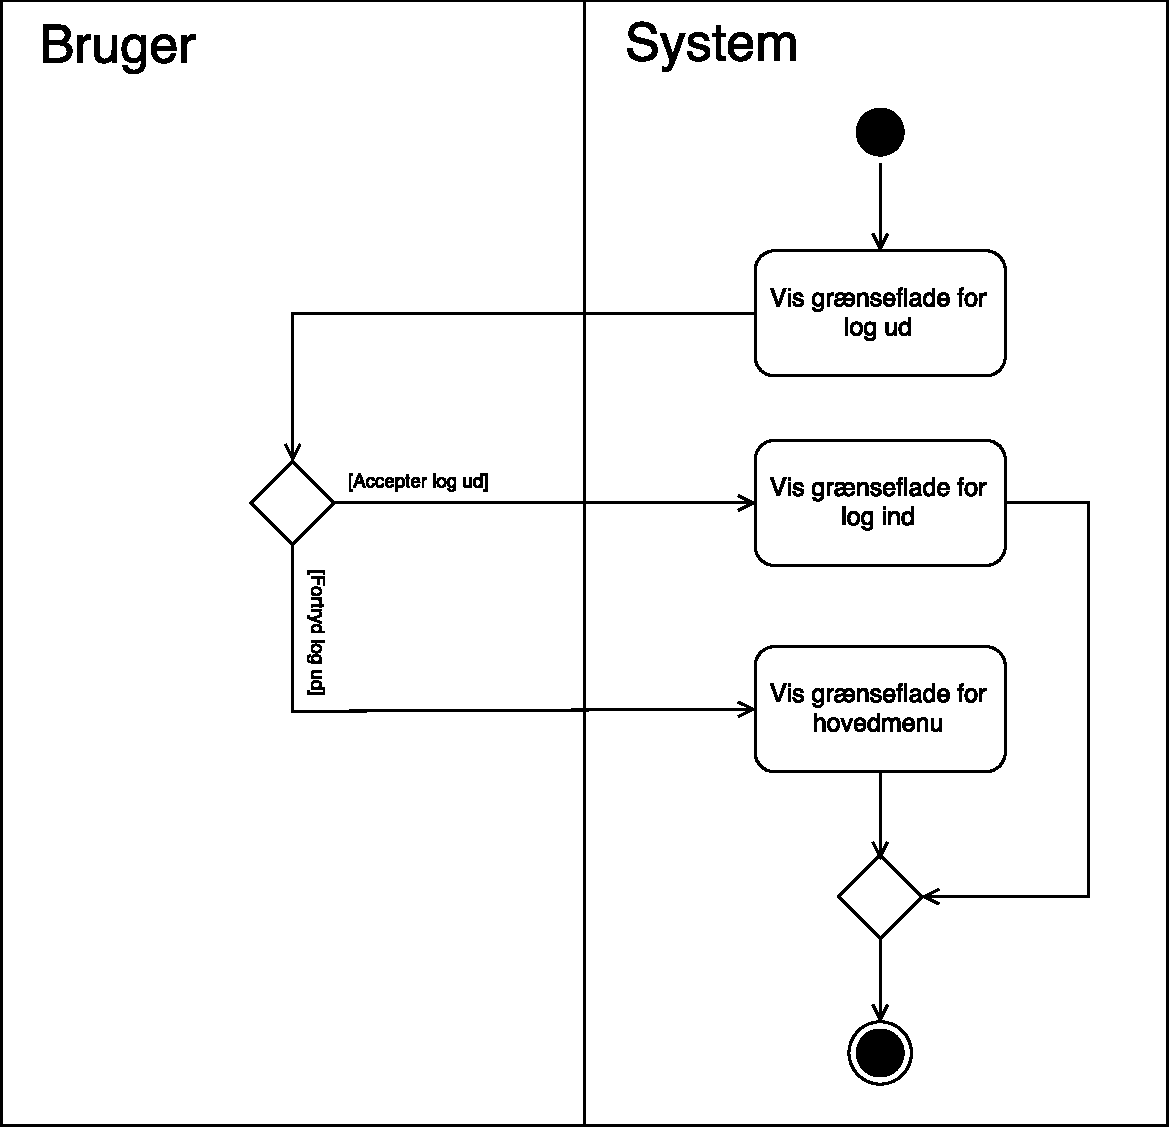
\includegraphics[width=0.6\textwidth]{figures/MVC/Logud}
\caption{Designklasser for log ud. Til venstre ses boundary og til højre controller.}
\label{fig:MVCLogUd}
\end{figure}

\noindent
Der opstilles i log ud et tekstfelt, af typen TextView. Dertil opstilles en BekræftKnap og FortrydKnap af typen Button. 
Den tilhørende controller indeholder private metoder Vis, Lyt, Logud og Start. Logud-metoden har til formål at slette data på app'en, hvorefter denne kan oprettes på ny, idet en bruger logger ind. 

I sammenspil med designklasserne er der opstillet et sekvensdiagram, som fremgår af \autoref{fig:SEKlogUd}.

\begin{figure} [H]
\centering
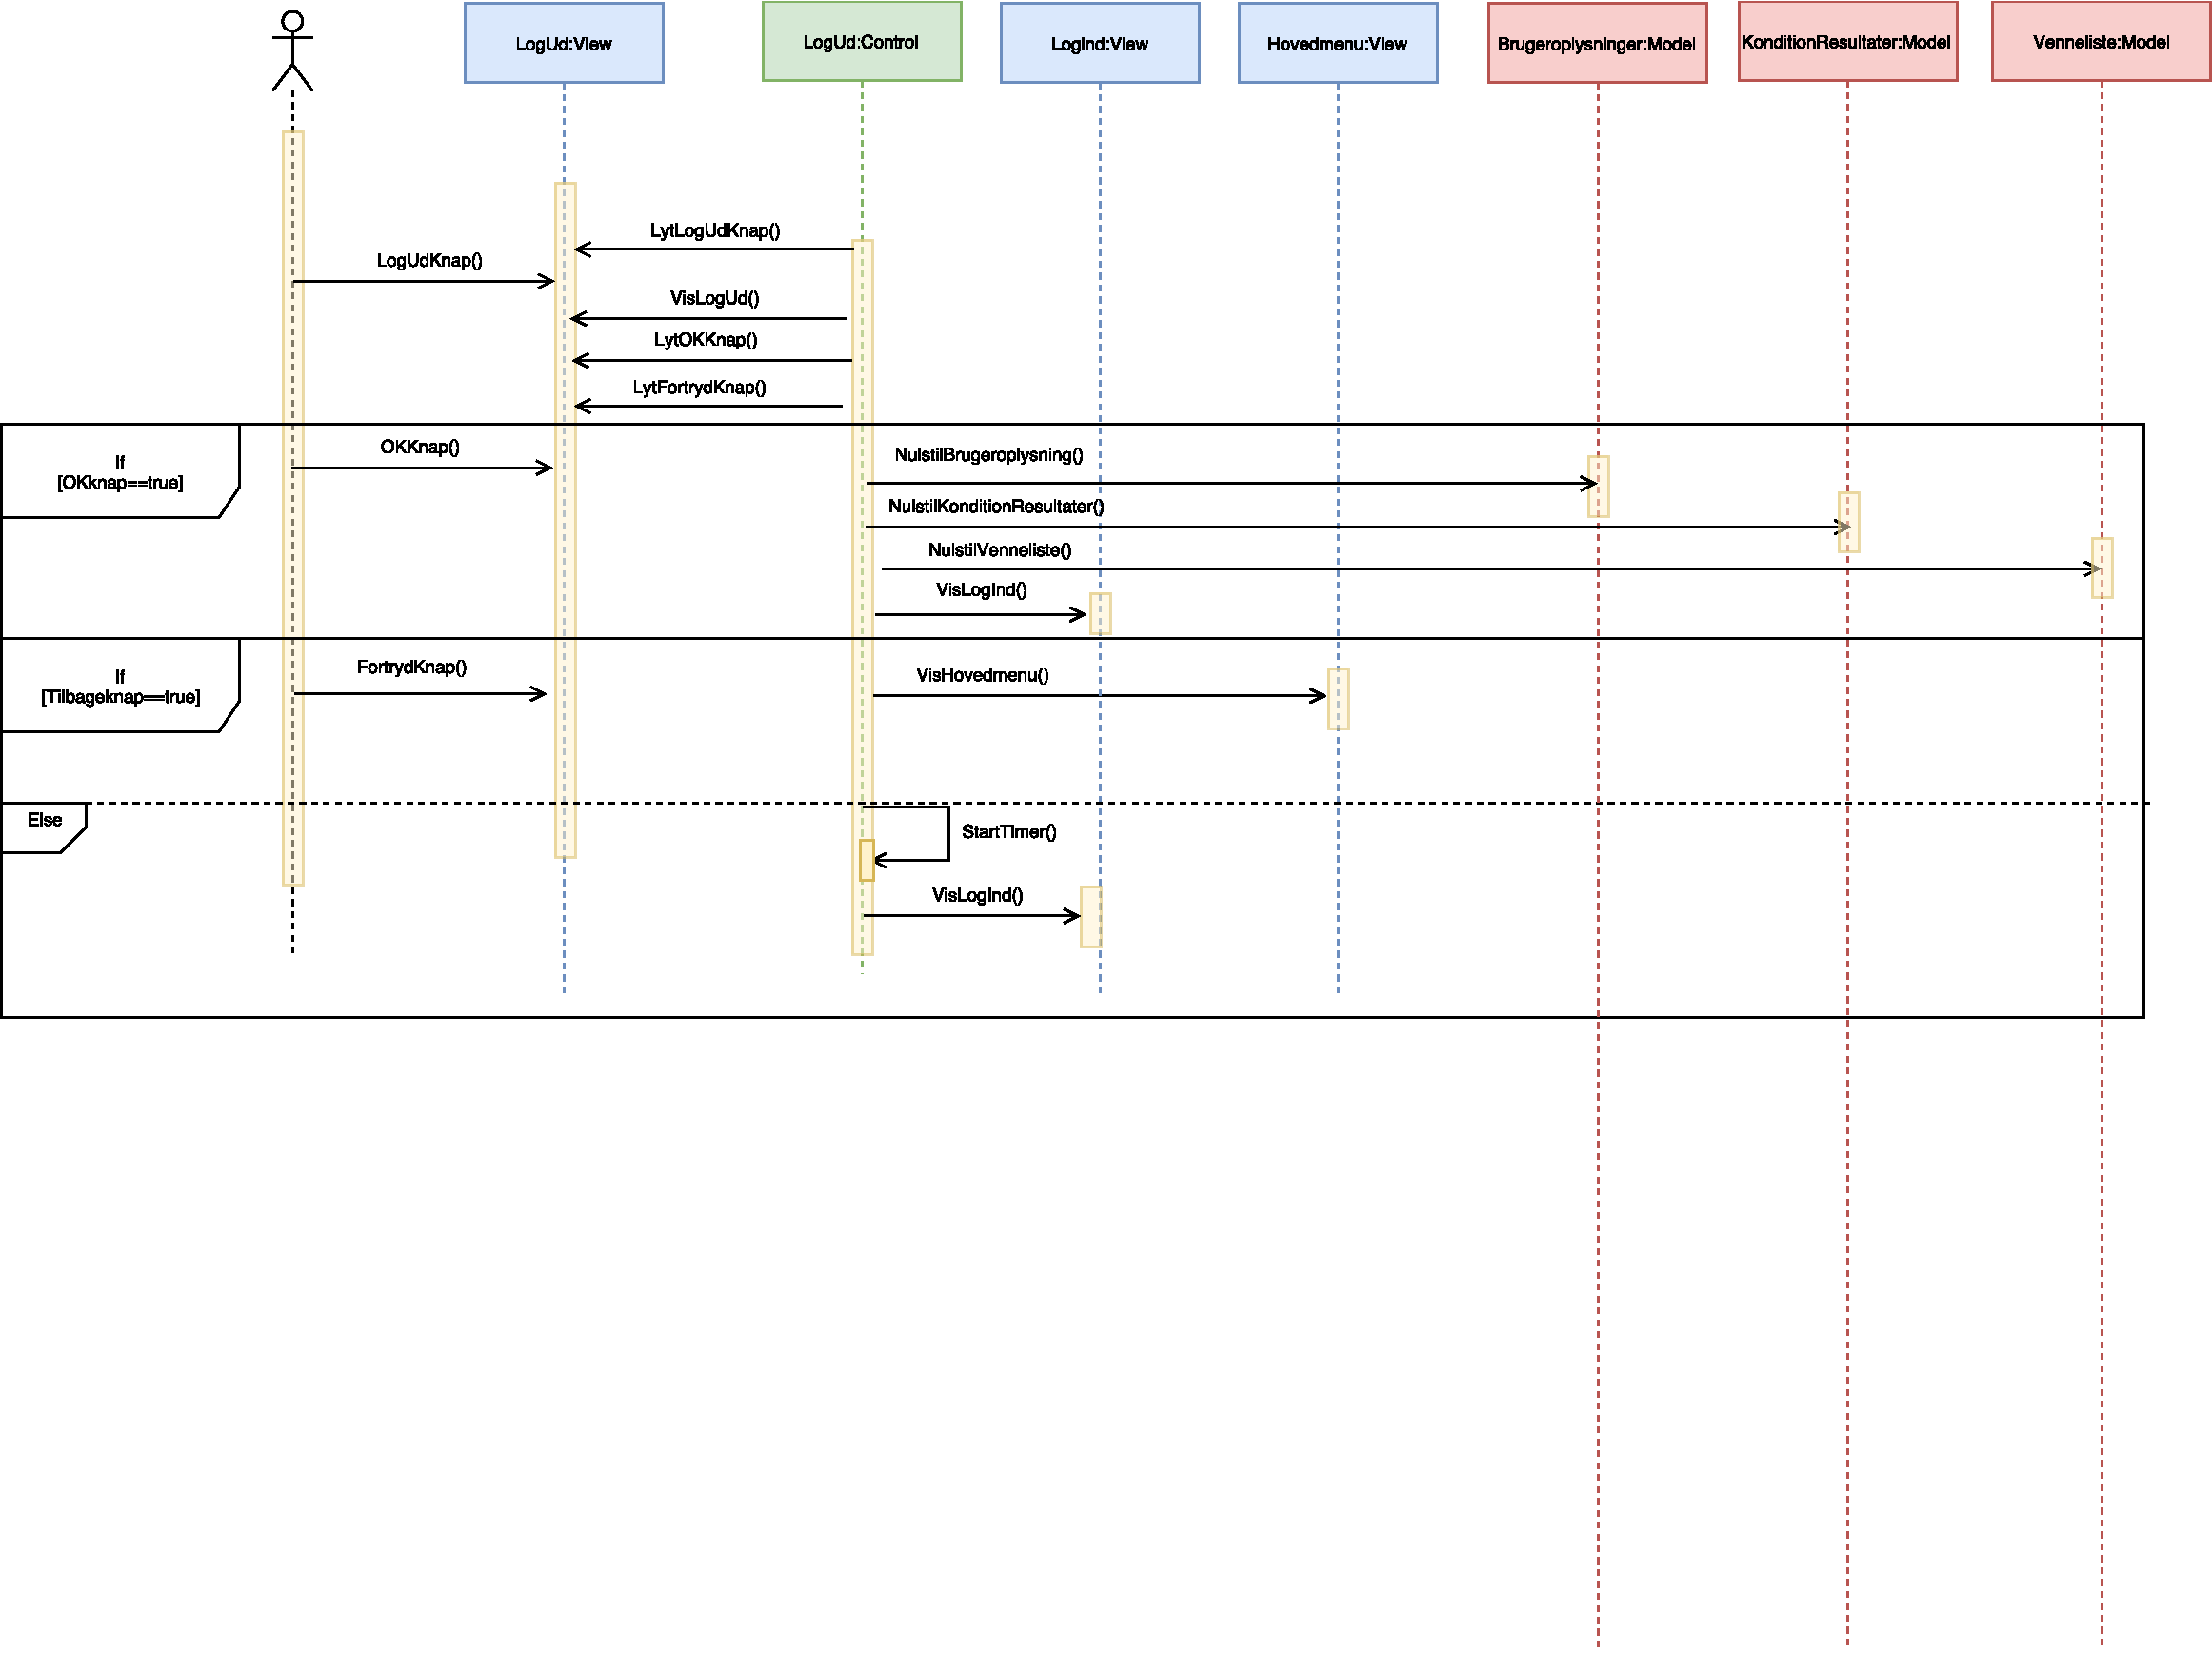
\includegraphics[width=1.28\textwidth]{figures/Sek/SEKLogUd}
\caption{Sekvensdiagram for log ud.}
\label{fig:SEKlogUd}\\
\end{figure}

\noindent
Når brugeren via hovedmenuen trykker på knappen for log ud vises grænsefladen for \textit{Log ud}. Her har brugeren mulighed for at trykke på BekræftKnap eller FortrydKnap. Hvis brugeren trykker på BekræftKnap, logges brugeren ud ved, at \textit{Brugeroplysninger} og \textit{KonditionResultater} destrueres, hvorefter grænsefladen for \textit{Log ind} vises. Trykker brugeren på FortrydKnap, vises grænsefladen for \textit{Hovedmenu} igen. 
